\chapter{Introduction}

\section{Differential Equations}
\subsection{Poisson's equation}

This is the introduction ~\cite{Example}.

A first demonstration is solving the Poisson equation, which is elliptic. For a domain
$ \Omega \subset \mathbb{R}^n $ with boundary $\partial \Omega = \Gamma_{D} \cup \Gamma_{N}$ the equation reads:

\begin{align}
  - \frac{d^2u(x)}{dx^2} = f(x) &, \\
  u(-1) = g &, u(1) = h,
\end{align}

giving a strong residual of
\begin{align}
  r(x) = - \frac{d^2u_{NN}(x)}{dx^2} - f(x), && x \in  (-1, 1) \\
  r_b(x) = u_{NN}(x) - u(x), && x = \pm 1
\end{align}

\begin{align}
  -\nabla^2 u   &= f  && \text{in $\Omega$,} \\
      u   &= 0  && \text{on $\Gamma_D$,} \\
  \nabla u \cdot n &= g  && \text{on $\Gamma_N$.}
\end{align}

\subsection{hp-FEM}
An extension of finite elements are the hp-Finite-Elements.
Which use quadratic elements, of width $h$. And a sum of polynomial functions of degree $p$. Used as the test function.

\subsection{Gauss-Lobatto Quadrature}

Gaussian quadrature has been used to approximate the result of integrals by the know function values in the desired range usually $[-1, 1]$ with the form

\begin{align}
  \int f(x)dx \approx \sum_{i=1}^{n} w_i f(x_i),
\end{align}

with $w_i$ being the appropriate weights. In Gauss-Lobatto quadrature, where the end points of the range are included in the integration. The nodes $x_i$ are selected from the zeros of the Legendre functions with degree $n$. The formula is given by:

\begin{align}
  \int f(x)dx = \frac{2}{n(n-1)}[f(1) + f(-1)] + \sum_{i=2}^{n-1} w_i f(x_i) + R_n.
\end{align}

with the weights given by

\begin{align}
  w_i = \frac{2}{n(n-1)[P_n-1 (x_i)]^2}, \qquad x \neq \pm 1
\end{align}

\section{Neural Networks}
Neural nets have had many successes with many computational problems in the last few years,
thanks to their ability to very quickly and in a parallel way to optimize certain problems. ~\cite{Example}

\begin{figure}[!ht]
  \centering
  \tikzset{%
  every neuron/.style={
    circle,
    draw,
    minimum size=0.65cm
  },
  neuron missing/.style={
    draw=none,
    scale=3,
    text height=0.222cm,
    execute at begin node=\color{black}$\vdots$
  },
}

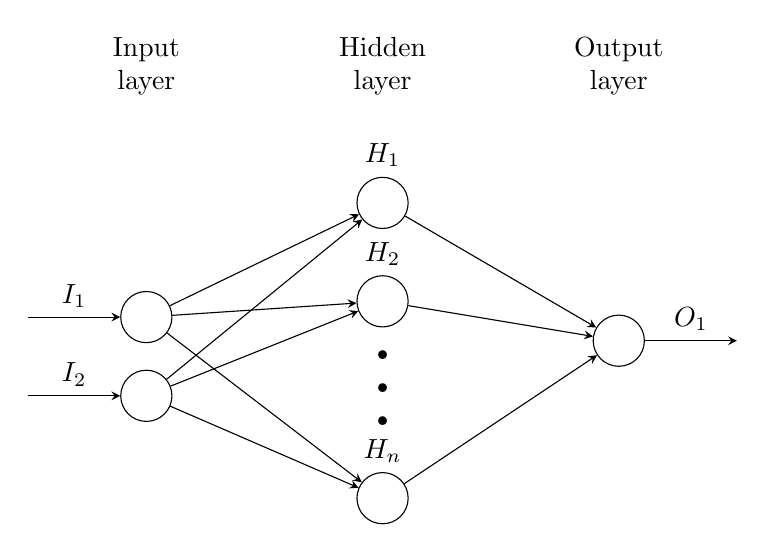
\begin{tikzpicture}[x=1.5cm, y=1.0cm, >=stealth]

\foreach \m/\l [count=\y] in {1,2}
  \node [every neuron/.try, neuron \m/.try] (input-\m) at (0,0.3-\y) {};

\foreach \m [count=\y] in {1,2,missing,3}
  \node [every neuron/.try, neuron \m/.try ] (hidden-\m) at (2,2-\y*1.25) {};

\foreach \m [count=\y] in {1}
  \node [every neuron/.try, neuron \m/.try ] (output-\m) at (4,0.0-\y) {};

\foreach \l [count=\i] in {1,2}
  \draw [<-] (input-\i) -- ++(-1,0)
    node [above, midway] {$I_\l$};

\foreach \l [count=\i] in {1,2,n}
  \node [above] at (hidden-\i.north) {$H_\l$};

\foreach \l [count=\i] in {1}
  \draw [->] (output-\i) -- ++(1,0)
    node [above, midway] {$O_\l$};

\foreach \i in {1,2}
  \foreach \j in {1,2,...,3}
    \draw [->] (input-\i) -- (hidden-\j);

\foreach \i in {1,2,...,3}
  \foreach \j in {1}
    \draw [->] (hidden-\i) -- (output-\j);

\foreach \l [count=\x from 0] in {Input, Hidden, Output}
  \node [align=center, above] at (\x*2,2) {\l \\ layer};

\end{tikzpicture}

\end{figure}

\section{Automatic Differentiation}

In order to obtain the required derivatives for the optimization process of a PINN, one could either resort to manually obtaining them and coding them, or numerically with a method such as central differences or symbolically where a program can manipulate expressions and provide a closed-form of the required function. ~\cite{Automatic}

All methods mentioned above are unsuitable for deep-learning applications .

Manual differentiation is very error prone, if not humanly-impossible for very deep nets.
Numerical differentiations of the form

\begin{align}
  \frac{\partial f(\mathbf{x})}{\partial x_i} \approx \frac{f(\mathbf{x} + h\mathbf{e}))}{h}
\end{align}

is easy to implement, but round-off and truncation errors make it unacceptable for the gradients of deep-learning problems, which can be dependent on millions of parameters.

Symbolic differentiation, addresses the issues of manual and numerical differentiation, but its expression can be complex and suffer from "expression swell", the time required to compute a derivative scales together with the complexity of the expression.

Automatic Differentiation (also known as \emph{algorithmic differentiation}) can tackle effectively the aforementioned issues.
Automatic Differentiation relies on the chain rule $(f \circ g)' = (f'\circ g)\cdot g'$consists of two modes, \emph{forward accumulation} and \emph{backward accumulation}, which dictate how one can reach $dy/dw_i$ from $dw_i/dx$ and vice versa.

\begin{figure}[!ht]
  \centering
  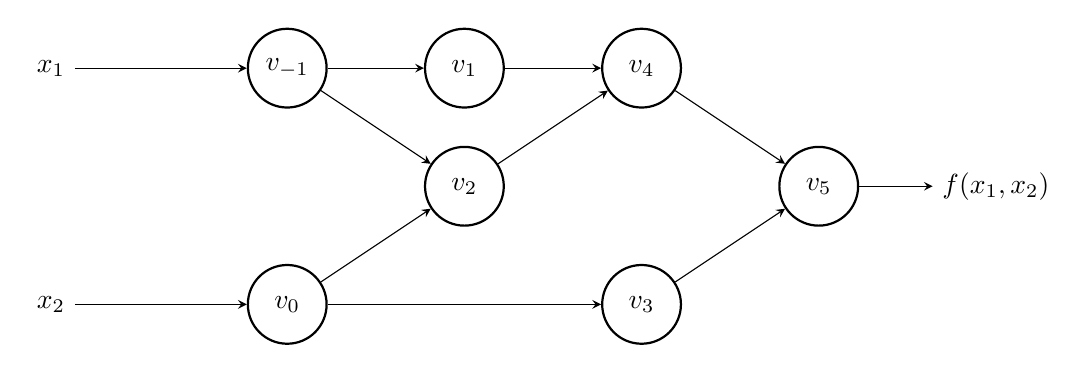
\begin{tikzpicture}[x=1.5cm, y=1.0cm, >=stealth]
\begin{scope}[]
    \node (x1) at (-2,1.5) {$x_1$};
    \node (x2) at (-2,-1.5) {$x_2$};
    \node (f) at (6,0) {$f(x_1, x_2)$} ;
\end{scope}

\begin{scope}[every node/.style={circle,thick,draw, minimum size=1cm}]
    \node (v-1) at (0,1.5)  {$v_{-1}$};
    \node (v1)  at (1.5,1.5)  {$v_1$};
    \node (v4)  at (3,1.5) {$v_4$};
    \node (v2)  at (1.5,0) {$v_2$};
    \node (v5)  at (4.5,0) {$v_5$};
    \node (v0)  at (0,-1.5) {$v_0$};
    \node (v3)  at (3,-1.5) {$v_3$};
\end{scope}

\begin{scope}[ ]
    \path [->] (x1) edge (v-1);
    \path [->] (v-1) edge (v1);
    \path [->] (v-1) edge (v2);
    \path [->] (v1) edge (v4);
    \path [->] (v2) edge (v4);
    \path [->] (v4) edge (v5);
    \path [->] (x2) edge (v0);
    \path [->] (v0) edge (v3);
    \path [->] (v0) edge (v2);
    \path [->] (v3) edge (v5);
    \path [->] (v5) edge (f);
\end{scope}
\end{tikzpicture}

  \caption{"The forward accumulation graph"}
\end{figure}


\section{Physics Informed Neural Networks}

Due to the overlap of the notation of "test" within Finite Element Analysis and Machine Learning,
to avoid any confusion in this work we will use the former unless explicitly told so.

\subsection{Residuals}

\begin{align}
  \mathcal{R}_{j}(\tilde{u}) &=  \int_{\Omega \times (0, T] } r(\tilde{u}) \varv_j dx = 0 \\
  \mathcal{R}_{b,j}(\tilde{u}) &=  \int_{\partial\Omega \times (0, T] } r_b(\tilde{u}) \varv_j dx = 0 \\
  \mathcal{R}_{0,j}(\tilde{u}) &=  \int_\Omega r_0(\tilde{u}) \varv_j dx = 0
\end{align}

\begin{align}
  \min_{\mathbf{W}, \mathbf{b}} \mathcal{J} (\tilde{u}, \varv),
\end{align}

where $\mathcal{J}$ is defined as

\begin{align}
  \mathcal{J} (\tilde{u}, \varv) = w \sum_{j=1}^{N_r} \mathcal{R}_j^{2} (\tilde{u}) + w_b \sum_{j=1}^{N_b} \mathcal{R}_{b,j}^{2} (\tilde{u}) + w_0 \sum_{j=1}^{N_0} \mathcal{R}_{0,j}^{2} (\tilde{u})
\end{align}

thus on a per-element basis we obtain the following variational loss:

\begin{align}
  L^p = \sum_{e=1}^{N_{el}}\frac{1}{K^{(e)}}\sum_{k=1}^{K^{(e)}}\left|\mathcal{R}_k^{(e)}\right|^2 + \tau_b\frac{1}{N_b}\sum_{i=1}^{N_b}\left|r_b(\mathbf{x}_b^i,\mathbf{r}_b^i)\right|^2 + \tau_0\frac{1}{N_0}\sum_{i=1}^{N_0}\left|r_0(\mathbf{x}_b^i)\right|^2
\end{align}
